\documentclass[12pt, border=8pt]{standalone}
\usepackage{tikz}
\usepackage{amsmath, amssymb, bm}
\usepackage{xcolor}
\usepackage{booktabs}
\usetikzlibrary{positioning, arrows.meta, calc, fit, backgrounds, 3d}

\begin{document}


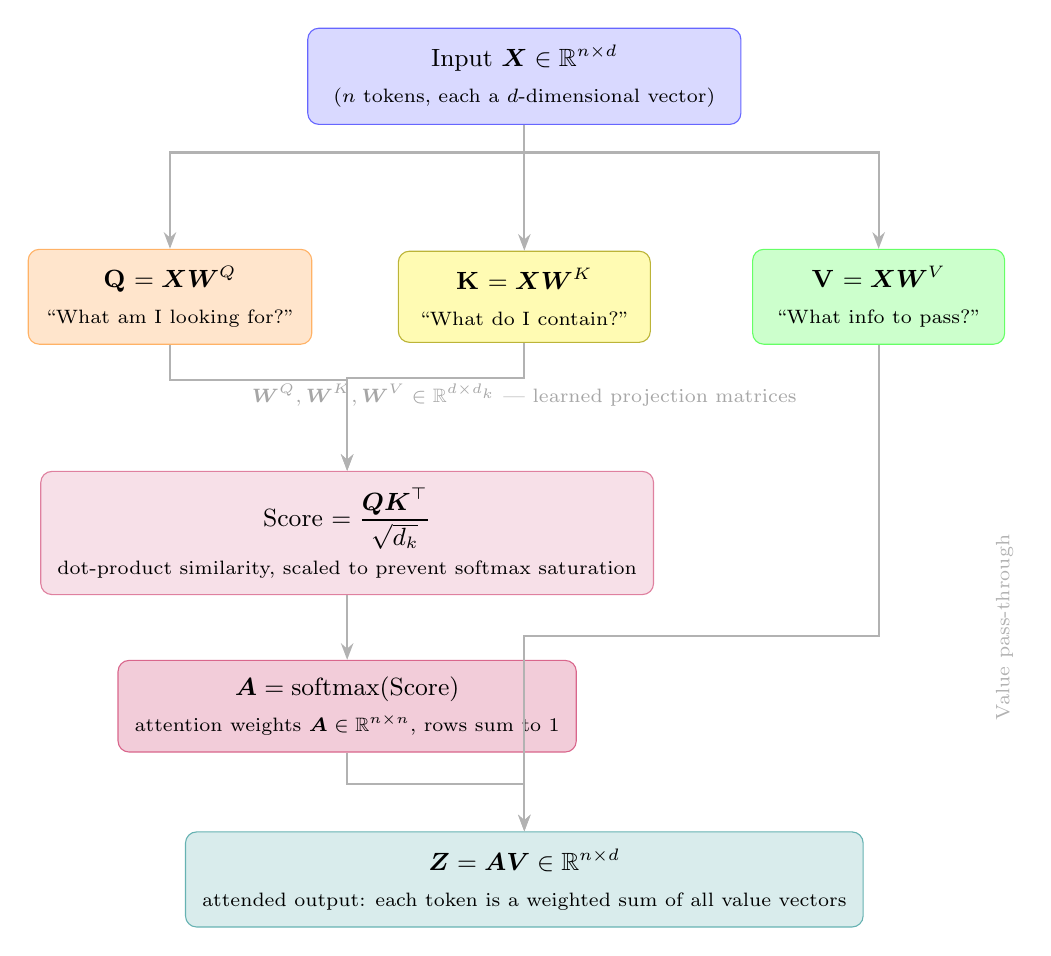
\begin{tikzpicture}[
  every node/.style={font=\small},
  arr/.style={-{Stealth[length=6pt]}, thick, gray!60},
  box/.style={draw, rounded corners=4pt, minimum width=5.5cm, minimum height=1.0cm,
              align=center, inner sep=6pt, font=\small},
  sbox/.style={draw, rounded corners=4pt, minimum width=3.2cm, minimum height=1.1cm,
               align=center, inner sep=6pt, font=\small}
]

%% 1. Input X
\node[box, fill=blue!15, draw=blue!60] (input)
  at (0,0) {Input $\bm{X} \in \mathbb{R}^{n \times d}$\\[2pt]
             {\scriptsize ($n$ tokens, each a $d$-dimensional vector)}};

%% 2a. Q projection
\node[sbox, fill=orange!20, draw=orange!60] (Q)
  at (-4.5,-2.8) {\textbf{Q} $= \bm{X}\bm{W}^Q$\\[2pt]
                  {\scriptsize``What am I looking for?''}};

%% 2b. K projection
\node[sbox, fill=yellow!30, draw=yellow!70!black] (K)
  at (0,-2.8) {\textbf{K} $= \bm{X}\bm{W}^K$\\[2pt]
               {\scriptsize``What do I contain?''}};

%% 2c. V projection
\node[sbox, fill=green!20, draw=green!60] (V)
  at (4.5,-2.8) {\textbf{V} $= \bm{X}\bm{W}^V$\\[2pt]
                 {\scriptsize``What info to pass?''}};

%% Shared note for weight matrices
\node[font=\scriptsize, align=center, text=gray!70] at (0,-4.05)
  {$\bm{W}^Q,\bm{W}^K,\bm{W}^V \in \mathbb{R}^{d \times d_k}$ --- learned projection matrices};

%% 3. Score box
\node[box, fill=purple!12, draw=purple!50] (score)
  at (-2.25,-5.8) {Score $= \dfrac{\bm{Q}\bm{K}^\top}{\sqrt{d_k}}$\\[3pt]
                   {\scriptsize dot-product similarity, scaled to prevent softmax saturation}};

%% 4. Softmax box
\node[box, fill=purple!20, draw=purple!60] (softmax)
  at (-2.25,-8.0) {$\bm{A} = \text{softmax}(\text{Score})$\\[2pt]
                   {\scriptsize attention weights $\bm{A} \in \mathbb{R}^{n \times n}$, rows sum to 1}};

%% 5. Output box
\node[box, fill=teal!15, draw=teal!60] (output)
  at (0,-10.2) {$\bm{Z} = \bm{A}\bm{V} \in \mathbb{R}^{n \times d}$\\[2pt]
                {\scriptsize attended output: each token is a weighted sum of all value vectors}};

%% ---- Arrows ----
% Input -> Q, K, V
\draw[arr] (input.south) -- ++(0,-0.35) -| (Q.north);
\draw[arr] (input.south) -- ++(0,-0.35) -| (K.north);
\draw[arr] (input.south) -- ++(0,-0.35) -| (V.north);

% Q -> Score
\draw[arr] (Q.south) -- ++(0,-0.45) -| (score.north);

% K -> Score
\draw[arr] (K.south) -- ++(0,-0.45) -| (score.north);

% Score -> Softmax
\draw[arr] (score.south) -- (softmax.north);

% Softmax -> Output
\draw[arr] (softmax.south) -- ++(0,-0.4) -| (output.north);

% V -> Output (from the right)
\draw[arr] (V.south) -- ++(0,-3.7) -| (output.north);

%% ---- Side label for V path ----
\node[font=\scriptsize, rotate=90, text=gray!60] at (6.1,-7.0) {Value pass-through};

\end{tikzpicture}

\end{document}
